To build and install microML ensure that \textbf{stack} is available on your system. 

\begin{figure}
    \label{fig:help}
    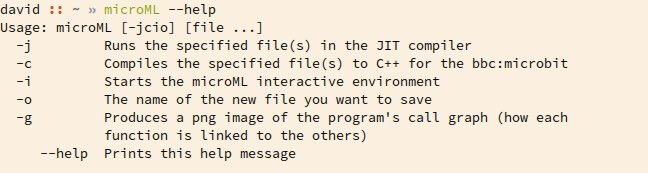
\includegraphics[width=\textwidth]{images/help.jpg}
    {\caption{MicroML command line help}}
\end{figure}

\begin{itemize}
    \item Download the repository from Git \url{https://github.com/kellino/microML}
    \item Unzip the repository and cd into the directory.
    \item Run `stack build' to create an executable or `stack test' to run the tests and build.
    \item Copy the executable into your system path.
\end{itemize}

MicroML expects to find the standard library in the home directory in a folder called `.microML'.
Create this directory and copy the files in Lib into it.

Typing `microML --help' into the terminal shows the various options. See Figure~\ref{fig:help}.


